\chapter{Methodology}
\label{Methodology}

The main paradigm used for this thesis is Design Science Research (DSR), as currently outlined by \textcite{brocke2020designscience}.
The author of this thesis used existing theories, frameworks, and models to produce and evaluate a new innovative artifact --- instantiation, as categorised by \textcite{hevner2004designscience}.

The created artifact is a web application --- referred to as "Proposed Software" for the rest of this thesis.
The most popular existing software that Proposed Software improves on is the Nand2Tetris Java desktop application\footnote{Available at \url{https://www.nand2tetris.org/software}.} --- referred to as "Existing Software" for the rest of this thesis.

This thesis aims to: show it is feasible for Proposed Software to effectively implement the same selected functionality on the client-side web; analyse the usability (and specifically efficiency) improvements compared to Existing Software; and explore the link between usability and efficiency.
As such, it starts with a description of the approach used to design Proposed Software.
After that, it covers the evaluation of Proposed Software consisting of the following:

\begin{itemize}
    \item \textbf{Functional Testing} to verify Proposed Software can perform the selected functions Existing Software can (feature parity of selected parts) and that it works as expected (correctness).
    \item \textbf{Comparative Study} to collect and analyse mainly quantitative and partially qualitative data on the efficiency and usability of Proposed Software and Existing Software while performing the same set of tasks under controlled conditions.
\end{itemize}

\section{Software Design}
\label{sec:software-design}

The design of the software tries to maximise the usability and accessibility of the software based on knowledge from sections on \gls{hci} Ergonomics: \Cref{Literature-HSIE-Benefits} and \Cref{Literature-HSIE-Implementation}.
As such, the chosen approach to technology choice kept in mind access from as many devices as possible, taking note of data from \Cref{sec:device-types} and for people with as many limitations as possible.
Moreover, considering some common problems when learning are lack of time and technical difficulties (see \Cref{sec:learning-state}), the chosen path was to streamline all interactions as much as possible.
To draw on the knowledge from \Cref{sec:text-code} and \Cref{sec:creating-application}, the design consciously incorporated covered computer science and software engineering practices.
Whenever possible, the design and implementation of Proposed Software is compared to Existing Software in terms of the chosen approach, its effects on the mentioned goals, or by using metrics.

The author chose to reuse existing \gls{oss} if it fulfilled the requirements mentioned above and if the short-term investment into custom solution would be greater than the time saved long-term.
To ensure Proposed Software is legally sound and reusable by others, it did not use any proprietary or copyleft parts (including the GPL-licensed Existing Software).
At the same time, it was determined all choices must allow for publication under a permissive Open Source license to maximise possible further reuse.
In the case of the adapted learning content specifically, since the original is available under the \gls{cc} BY-NC-SA 3.0 license\footnote{See \url{https://www.nand2tetris.org/license}}, the adapted content had to use the same license.
Any chosen technologies, tools, and services had to be free (at least free of charge if not open) and relatively easy to use to improve reproducibility.

\section{Functional Testing}

Multiple types of automated tests were utilized to verify the functionality of Proposed Software.

\textbf{Unit Tests} were used for the verification of granular parts of the software with clear inputs and outputs.
That includes all proposed parsers that accept a text on the input and provide an \gls{ast} on the output; a factory that accepts an \gls{ast} on the input and produces chips on the output; elementary built-in and simple custom chips that have a clear interface and a definite number of combinations of inputs and outputs; and other similar reusable abstractions.
The exact unit test framework chosen for this purpose was Vitest\footnote{Available at \url{https://vitest.dev/}.}, as it is well-integrated with the code bundler Vite\footnote{Available at \url{https://vitejs.dev/}.} the chosen SvelteKit framework\footnote{Available at \url{https://kit.svelte.dev/}.} is based on.
The expected coverage on all files providing the mentioned functionality should exceed 80\%, which corresponds to the median coverage on projects at Google and is set to prevent an exponential increase in effort required to increase coverage further --- see \Cref{Literature-Software-Testing}.

\textbf{End-to-End UI Tests} verified the software from the viewpoint of a user.
In contrast to the Unit Tests, that meant designing automated tests that covered interaction between multiple components and even multiple screens.
Examples include navigation through Proposed Software with checks for the existence of essential information, interaction with the \gls{ide}, or error handling.
The tool of choice for this purpose was Cypress\footnote{Available at \url{https://www.cypress.io/}.}.
No automated coverage as a percentage was calculated for this group of automated tests, as many lines of code would be marked as covered (given the nature of these tests) even though they were not actively tested.
Instead, all major paths through the software (use cases) were identified and captured in an automated test unless the return on the effort to do so would not be considered worth it.
The reasoning was captured individually for each use case that was not covered.

\textbf{Accessibility Tests} checked automatically for common errors with incorrectly implemented \gls{api}[s] --- aiming for "technical accessibility" as mentioned in \Cref{Kinds-of-Accessibility}.
The chosen conformance target was "generally accepted and recommended" \gls{wcag} Level AA \parencite{WAI_Evaluation_Methodology_Note} and \gls{wcag} version 2.1 as it is the latest supported version within the \gls{wcagem} Report Tool as of the time of writing.
Checks were run on multiple screens in multiple states entered during the execution of Cypress tests to test for possible violations continually and in more scenarios than can be realistically achieved using one-off evaluation.
This was accomplished using the \gls{js} package cypress-axe that integrates aXe --- an accessibility testing engine that powers Google's Lighthouse as mentioned in \Cref{Accessibility-Tools}.
Considering the limited amount of time and resources, the human testing involved was limited to testing done by the author to produce the \gls{wcagem} report.

The actual extent and output from all mentioned types of tests, including additional information, where relevant, was captured in \Cref{Evaluation-Tests}.

\section{Comparative Study}

The central hypothesis is that using Proposed Software instead of Existing Software will increase efficiency.
Therefore, the main objective of the comparative study was to perform summative testing of Existing Software and Proposed Software in a way that produces comparable data.
To do that, the author conducted a remote moderated usability testing and performed a between-subjects comparison.

The chosen methodology considers three kinds of variables to achieve conditions that would lead to the collection of comparable data:

\begin{itemize}
    \item \textbf{Controlled} variables: for example, presented learning content, participant's profile, and actions performed outside of the measured software.
    \item \textbf{Independent} variable: the used software --- Existing Software or Proposed Software.
    \item \textbf{Dependent} variables: mainly the time spent on the tasks and the perceived usability.
\end{itemize}

Since the only independent variable is the used software and there are two options, participants were split into two groups:

\begin{itemize}
    \item \textbf{Group A} using Proposed Software.
    \item \textbf{Group B} using Existing Software.
\end{itemize}

Target users of the software are expected to come from different backgrounds corresponding to three target demographics mentioned in \Cref{Introduction}: \gls{cs} students, practitioners with/without formal education, and people interested, but not directly involved, in Computer Science.
Participants were recruited from the social circle of the author, and they were subsequently asked if they knew any other potentially interested participants.
To control for external motivation and help with the recruitment, one-half of participants within both groups were paid to participate at a rate of 10 euros per hour, as suggested by Prolific\footnote{Archived Prolific calculator: \url{https://web.archive.org/web/20221221162903/https://app.prolific.co/calculator.html}}.
However, Prolific or a similar crowdsourcing method was not used to recruit participants.
All participants were based in an advanced economy country as defined by the International Monetary Fund\footnote{Available at \url{https://www.imf.org/external/pubs/ft/weo/2022/01/weodata/groups.htm}.}.
Almost all participants were non-native English speakers.

Participants were pre-screened to make sure they:
\begin{itemize}
    \item Are capable of reading English text of an academic nature.
    \item Are at least somehow interested in \gls{ict} and either want to pursue a career in the field or are already active in the field.
    \item Have a suitable device to run desktop software.
    \item Can join a Google Meet voice call and share their screen.
\end{itemize}

\subsection{Controlled Variables}

Both groups used the same simplified content based on the \gls{cc}[-licensed] Nand2Tetris content from \textcite{nand2tetris}.
After several rounds of pilot studies, the content and assigned tasks were simplified significantly to reduce the time needed to complete the session and to control for the differences in the ability to learn new concepts.
As a result, the tasks were mostly mechanical in nature and could be performed just by using the same set of steps that were shown in an example.
In the end, participants were expected to spend more time with the software and less time learning and thinking about the presented problems.

The learning material consisted of the same short introduction to Boolean algebra and Boolean gate logic and design.
As part of the content, there was a video showing how to solve the first example that differed only in the necessary parts that involved the tested software.

The study was conducted by the author using the same online meeting software, Google Meet.
Each participant took the comparative study individually so that the author could fully focus on only one person, and other people did not influence the results.

All participants used their own devices, with only laptops and desktop computers allowed due to the limitations of Existing Software --- a desktop Java software.
The use of the participant's device aims to reflect how target users are likely to practice, work on assignments, or explore the content on their own.

To lower the chances the participant would associate the content presented with the author that conducted the study:

\begin{itemize}
    \item All mentions of the author's name and website header with logo and navigation were removed from the modified version.
    \item Both videos featured a voice-over from the same professional voice actor with a neutral American accent, slow rate of speech, and clear pronunciation.
\end{itemize}

The communication between the participant and the author was kept to a minimum and consisted of the following:

\begin{enumerate}
    \item The participant is greeted and asked whether they are aware of the author's research or if they have heard any details about the comparative study from other participants.
    \item The author explains the participant will read a short text, watch a video, and will be expected to complete all presented tasks.
    \item The participant is asked to share their screen, and they are informed the screen recording will be kept only until all data are captured and that it will not be shared with any third party.
    \item The participant is asked to work on their own and to ask questions only if necessary.
    \item The author answers any questions the participant has after the learning content has loaded but before the participant dedicates their attention to the content.
    \item The author is strictly muted anytime they are not needed. If necessary, the author answers questions or offers help while the participant solves assigned tasks. This is typically noted in the captured data, as explained when describing dependent variables.
    \item After the participant finishes all of the assigned tasks, the author reminds the participant to use the link to open the administered \gls{sus} questionnaire. The participant is asked to be as objective as possible, reminding them there are no correct answers and that since the participant does not know which group they belong to, they should not try to knowingly influence the results either way.
\end{enumerate}

Since it is impossible to keep the profile of the participant the same if different groups of target users are to be represented, the author captured the following variables forming the participant's profile:

\begin{itemize}
    \item \textbf{Prior Experience} with the relevant topics on a scale of 0 to 2:
        \begin{itemize}[]
            \item \textbf{0} --- No prior experience.
            \item \textbf{1} --- Came into contact with the mentioned topics for a short period of time.
            \item \textbf{2} --- Has either relevant professional experience or was exposed to the topics for a long period of time.
        \end{itemize}
    \item \textbf{Education} in the field of Computer Science or Computing on a scale of 0 to 2:
    \begin{itemize}[]
        \item \textbf{0} --- No relevant education.
        \item \textbf{1} --- Taken modules included Boolean logic or programming in general, but not logic gates or chip design.
        \item \textbf{2} --- Learnt about Boolean gates and chip design specifically.
    \end{itemize}
    \item \textbf{Relevancy of Occupation} performed by the participant currently or recently on a scale of 0 to 2:
    \begin{itemize}[]
        \item \textbf{0} --- No relevant occupation.
        \item \textbf{1} --- Works as a part-time hardware designer, software developer or similar.
        \item \textbf{2} --- Works as a full-time hardware designer, software developer or similar.
    \end{itemize}
    \item \textbf{Intrinsically Motivated} to participate, as observed by the author on a scale of 0 to 2:
    \begin{itemize}[]
        \item \textbf{0}: Shows no significant interest in the topic. Is hesitant to start reading.
        \item \textbf{1}: Shows some interest in the topic and appears mostly focused.
        \item \textbf{2}: Is visibly engaged and explicitly confirms their interest in the topic.
    \end{itemize}
    \item \textbf{Paid} to participate:
    \begin{itemize}[]
        \item \textbf{1}: Yes.
        \item \textbf{0}: No.
    \end{itemize}
    \item \textbf{Age} on a scale of 18 to 65+:
    \begin{itemize}[]
        \item \textbf{18--29}
        \item \textbf{30--49}
        \item \textbf{50--64}
        \item \textbf{65+}
    \end{itemize}
    \item \textbf{Platform}:
    \begin{itemize}[]
        \item \textbf{Windows}: One of the commonly used desktop Windows NT versions --- Windows 7, Windows 8, Windows 10, or Windows 11.
        \item \textbf{Linux}: One of the currently supported versions of any commonly used distribution that uses a floating window manager like X11 or Wayland.
        \item \textbf{macOS}: One of the currently supported versions, regardless of the CPU architecture --- x86 or arm64.
    \end{itemize}
\end{itemize}

An effort was made to distribute participants among Group A and Group B so that their profiles are distributed equally.
Any correlations between these profile variables and dependent variables were analysed and revealed during the analysis of the results to hint at possible data skew.

\subsection{Independent Variable}

The link shared with Group A was \href{https://side-a.chipsandcode.pages.dev/}{side-a.chipsandcode.pages.dev}\footnote{Archived at \url{https://web.archive.org/web/20230810031115/https://side-a.chipsandcode.pages.dev/}} and the link shared with Group B \href{https://side-b.chipsandcode.pages.dev/}{side-b.chipsandcode.pages.dev}\footnote{Archived at \url{https://web.archive.org/web/20230810031153/https://side-b.chipsandcode.pages.dev/}}.

The use of Proposed Software by Group A and Existing Software by Group B was reflected mainly in the way tasks were assigned.
Group A had Proposed Software embedded within the same page with the assignment preloaded, as can be seen in Figure~\ref{fig:group-a-software}.
Group B, on the other hand, considering the limitations of Existing Software, had to start by copying three files representing the same assignment, as can be seen in Figure~\ref{fig:group-b-software}.

\begin{figure}[ht]
    \centering
    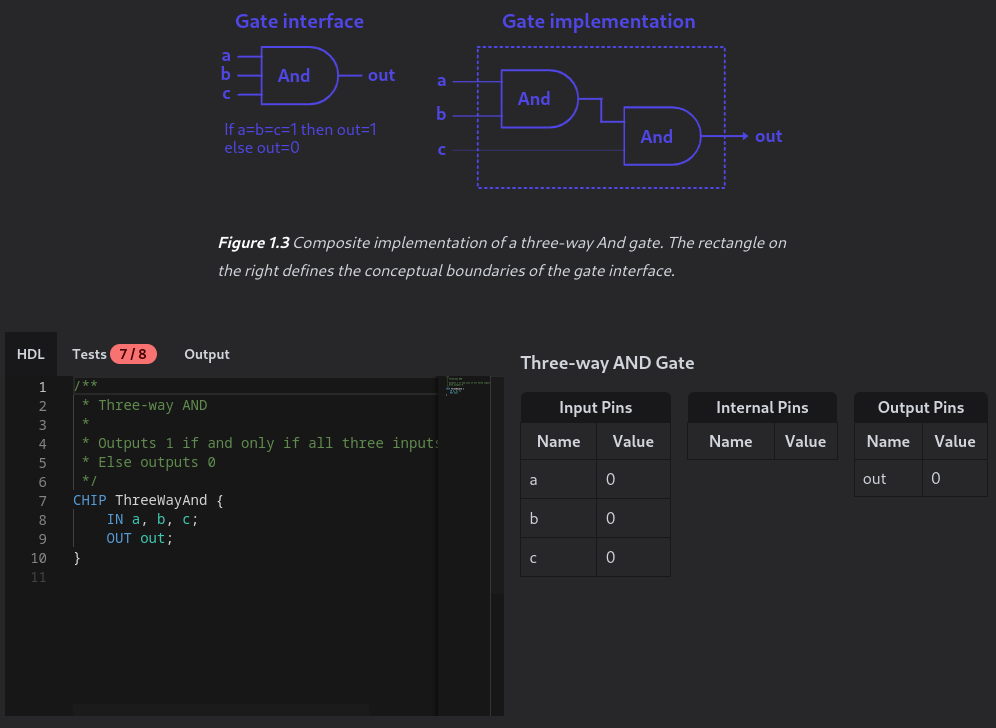
\includegraphics[height=8cm, keepaspectratio]{Group_A_Software}
    \caption{Screenshot of Proposed Software within text --- Group A.}
    \label{fig:group-a-software}
\end{figure}

\begin{figure}[ht]
    \centering
    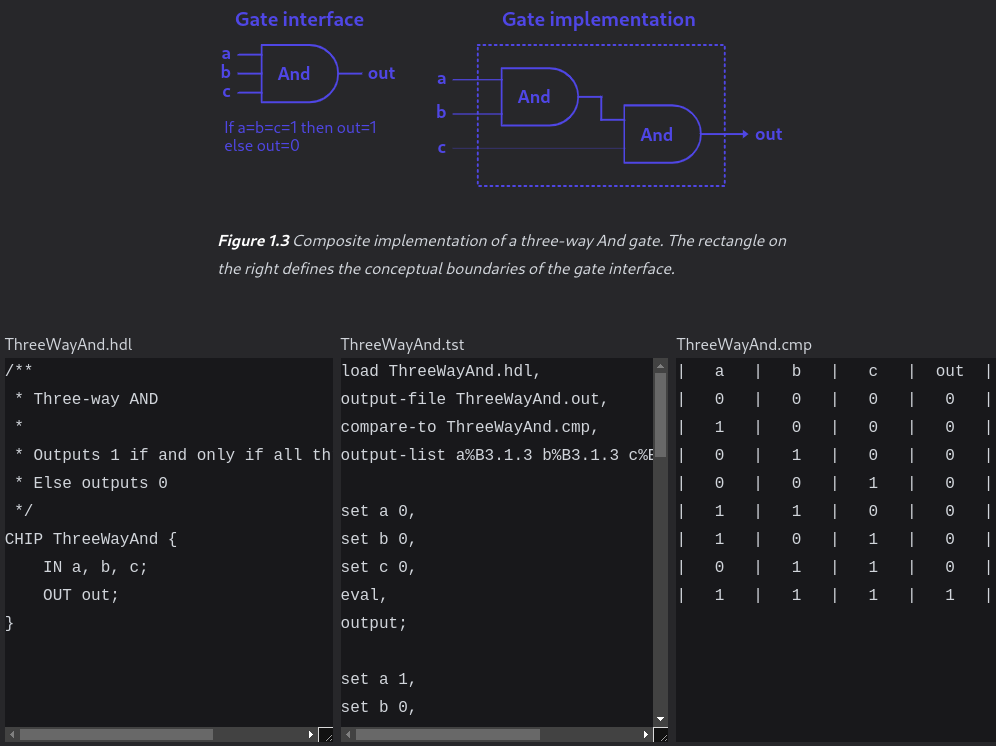
\includegraphics[height=8cm, keepaspectratio]{Group_B_Software}
    \caption{Screenshot of Existing Software's input within text --- Group B.}
    \label{fig:group-b-software}
\end{figure}

\subsection{Dependent Variables}
\label{sec:methodology-dependent-variables}

The following metrics were measured:

\begin{itemize}
    \item \textbf{Success} --- Did the participant complete all assigned tasks --- 1/0.
    \item \textbf{Preparation Time} --- Time required to start working with the hardware simulator in seconds. This includes the download and installation time in the case of Existing Software.
    \item \textbf{Time for 1st Task} --- Time required to finish the implementation of a three-way And Boolean gate in seconds.
    \item \textbf{Time for 2nd Task} --- Time required to finish the implementation of a Nand Boolean gate in seconds.
    \item \textbf{Time for 3rd Task} --- Time required to finish the implementation of a Nor Boolean gate in seconds.
    \item \textbf{Time for 4th Task} --- Time required to finish the implementation of a three-way Or Boolean gate in seconds.
    \item \textbf{Confusions} --- Number of times:
    \begin{enumerate}[(a)]
        \item The participant asked for help because they were confused.
        \item The author offered help to the participant because the participant had been stuck on the same problem for more than about one minute without any progress.
        \item The participant did not perform the needed action in the \gls{ui} due to a misunderstanding and could not immediately correct themselves.
    \end{enumerate}
\end{itemize}

The time it took the participant to initially go through the learning material and the embedded video was not measured and was excluded from the metrics mentioned above.
The time to perform a task was measured from the moment the participant started focusing on the part of the website that contains the task to the time they left the hardware simulator after all comparisons and optional manual testing was done.
These times were manually extracted by writing down the timestamp ranges from the screen recording after the session ended, an example of which can be seen in Table~\ref{table:timestamps}.

\begin{table}[!ht]
    \centering
    \caption{Partial timestamp data collected from one of the sessions.}
    \label{table:timestamps}
    \begin{tabular}{|l l|l|}
        \hline
        \textbf{Prep} & & \\ \hline
        \textbf{From} & \textbf{To} & \textbf{Time} \\ \hline
        0:10:45 & 0:12:25 & 0:01:40 \\ \hline
        0:13:32 & 0:15:06 & 0:01:34 \\ \hline
        ~ & \textbf{Total:} & \textbf{194} \\ \hline
        ~ & ~ & ~ \\ \hline
        \textbf{First Task} & ~ & ~ \\ \hline
        \textbf{From} & \textbf{To} & \textbf{Time} \\ \hline
        0:23:13 & 0:25:11 & 0:01:58 \\ \hline
        0:25:35 & 0:25:55 & 0:00:20 \\ \hline
        0:29:10 & 0:30:33 & 0:01:23 \\ \hline
        ~ & \textbf{Total:} & \textbf{221} \\ \hline
    \end{tabular}
\end{table}

While there was no hard time limit, the participant was informed the session would take one hour and was given the option to quit once the allocated time had passed.
The chosen approach to time limit aims to represent the way learners at home either have an expectation of how long the task will take or have allocated some time to the task but are willing to go past it if they feel like they are making progress and are close to finishing.

In addition to the mentioned metrics, participants were also asked to fill out the \gls{sus} \parencite{brooke_sus_1996} questionnaire using a 5-point Likert scale from Strongly agree to Strongly disagree.
This questionnaire was chosen based on the amount of supporting data combined with the relatively short length of 10 questions and the relevance of questions to the tested software.
The word "cumbersome" was replaced with the word "awkward" to help non-native speakers, see \Cref{sec:sus-evaluation}.

In the process, unstructured qualitative data were collected.
While the comparison did not primarily concentrate on qualitative data, it was mentioned when discussing relevant outcomes or theories in \Cref{Discussion}.
The collected qualitative edata included:

\begin{itemize}
    \item Explanations of confusing situations experienced by participants,
    \item Overall description of the experience of participants using the system,
    \item Various feedback.
\end{itemize}

\subsection{Data Analysis}
\label{sec:methodology-data-analysis}

To decrease the likelihood of manual errors when evaluating \gls{sus} scores, the author obtained the SUS Guide \& Calculator Package\footnote{Available at: \url{https://measuringu.com/product/suspack/}.}.
Based on \Cref{sec:sus-evaluation}, it was suggested at least 12 participants per group would need to participate in the study if the assumption is the effect size is relatively large.

The measured efficiency is represented by calculating the arithmetic mean of the measured times --- individually for each task and added together, and the mean number of confusions.
The subjective usability is analysed as a mean of \gls{sus} scores for each group.
Analysed data are assumed to follow standard distribution and all relevant calculations are done with two-tailed tests.

To determine the stastitical power of the gathered data, the results were evaluated using the two-sample $t$-test and included:

\begin{itemize}
    \item $p$-value, with expected $p \leq 0.1 $, ideally $p \leq 0.05 $,
    \item and confidence intervals.
\end{itemize}

Since the make-up of the groups was not identical, any profile variables that differed considerably were analysed for correlation with the dependent variables using Pearson's correlation coefficient.
As the assigned software is assumed to have a strong influence on the dependent variables, correlations are determined for each group individually with:

\begin{itemize}
    \item $|r| \le 0.2$ considered as no correlation,
    \item $0.2 < |r| \le 0.4$ considered as a weak correlation,
    \item $0.4 < |r| \le 0.6$ considered as a moderate correlation,
    \item $0.6 < |r|$ considered as a strong correlation.
\end{itemize}

Visually, results are presented using a series of charts and plots\footnote{Created using Plotly.js available at \url{https://plotly.com/javascript/}.}:

\begin{itemize}
    \item A linear chart with the time each group needed to perform subsequent tasks.
    \item A stacked bar chart showing the difference in measured efficiency.
    \item A box plot representing the mean and dispersion of the number of times participants got confused using each software.
    \item A box plot and a position on a percentile curve for \gls{sus} scores inspired by visualisations from \textcite{Blattgerste_2022}.
    \item A scatter plot showing the relation between the measured efficiency and \gls{sus} score, including colour-coding representing the group to reveal clusters.
    \item Scatter plots that show possible correlations between the various data points in participant profiles and dependent variables.
\end{itemize}

\subsection{Limitations}

The comparative study had several notable design limitations which could not be completely addressed:

\begin{itemize}
    \item \textbf{Sampling Bias}: The study participants consisting primarily of the extended social circle of the author and only includes participants who agreed to participate (self-selection bias).
    \item \textbf{Additional Step}: While Existing Software bundle does include a starting point for projects, it does not include the simple exercises chosen for this study. That means Group B participants had to take one extra step to create starting files.
    \item \textbf{Moderator Bias}: The study was moderated by the author rather than a blind data collector.
\end{itemize}
